\chapter{افراز اولیه‌ی \lr{k-means++} برای \lr{GLKM}}

\section{صورت دقیق ایده}

در نسخه‌ی اصلی \lr{GLKM} هر نقطه یک خوشه‌ی تک‌عضوی است؛ بنابراین برای رسیدن
به $k$ خوشه تقریباً $n-k$ ادغام لازم است. ایده‌ی آزمایش‌شده آن بود که ابتدا
$m=\alpha k$ خوشه بسازیم و سپس \lr{GLKM} را از این افراز آغاز کنیم تا فقط
$m-k$ ادغام انجام شود.

\section{نتایج مقدماتی روی \lr{Gisette}}

آزمایش نخست با $k=2$ و گراف ۸۰-نزدیک‌ترین همسایه انجام شد. جدول \ref{tab:kpp-fast} زمان کل و
معیارهای بیرونی را نشان می‌دهد.

\begin{table}[H]
    \centering
    \caption{اثر اندازه‌ی افراز اولیه؛ عبارت $10k$ یعنی آغاز از ۲۰ خوشه}
    \label{tab:kpp-fast}
    \begin{tabular}{lrrrr}
        \toprule
        آغاز          & زمان کل (ثانیه) & هزینه‌ی تقریبی ($10^7$) & \lr{ACC}   & \lr{NMI}   \\
        \midrule
        تک‌عضوی (اصلی) & \lr{1.33}       & \lr{2.586}             & \lr{0.795} & \lr{0.358} \\
        $4k$          & \lr{2.78}       & \lr{2.562}             & \lr{0.577} & \lr{0.033} \\
        $10k$         & \lr{3.28}       & \lr{2.561}             & \lr{0.748} & \lr{0.210} \\
        $25k$         & \lr{3.73}       & \lr{2.561}             & \lr{0.588} & \lr{0.054} \\
        $100k$        & \lr{10.87}      & \lr{2.563}             & \lr{0.760} & \lr{0.269} \\
        \bottomrule
    \end{tabular}
\end{table}

\begin{figure}[H]
    \centering
    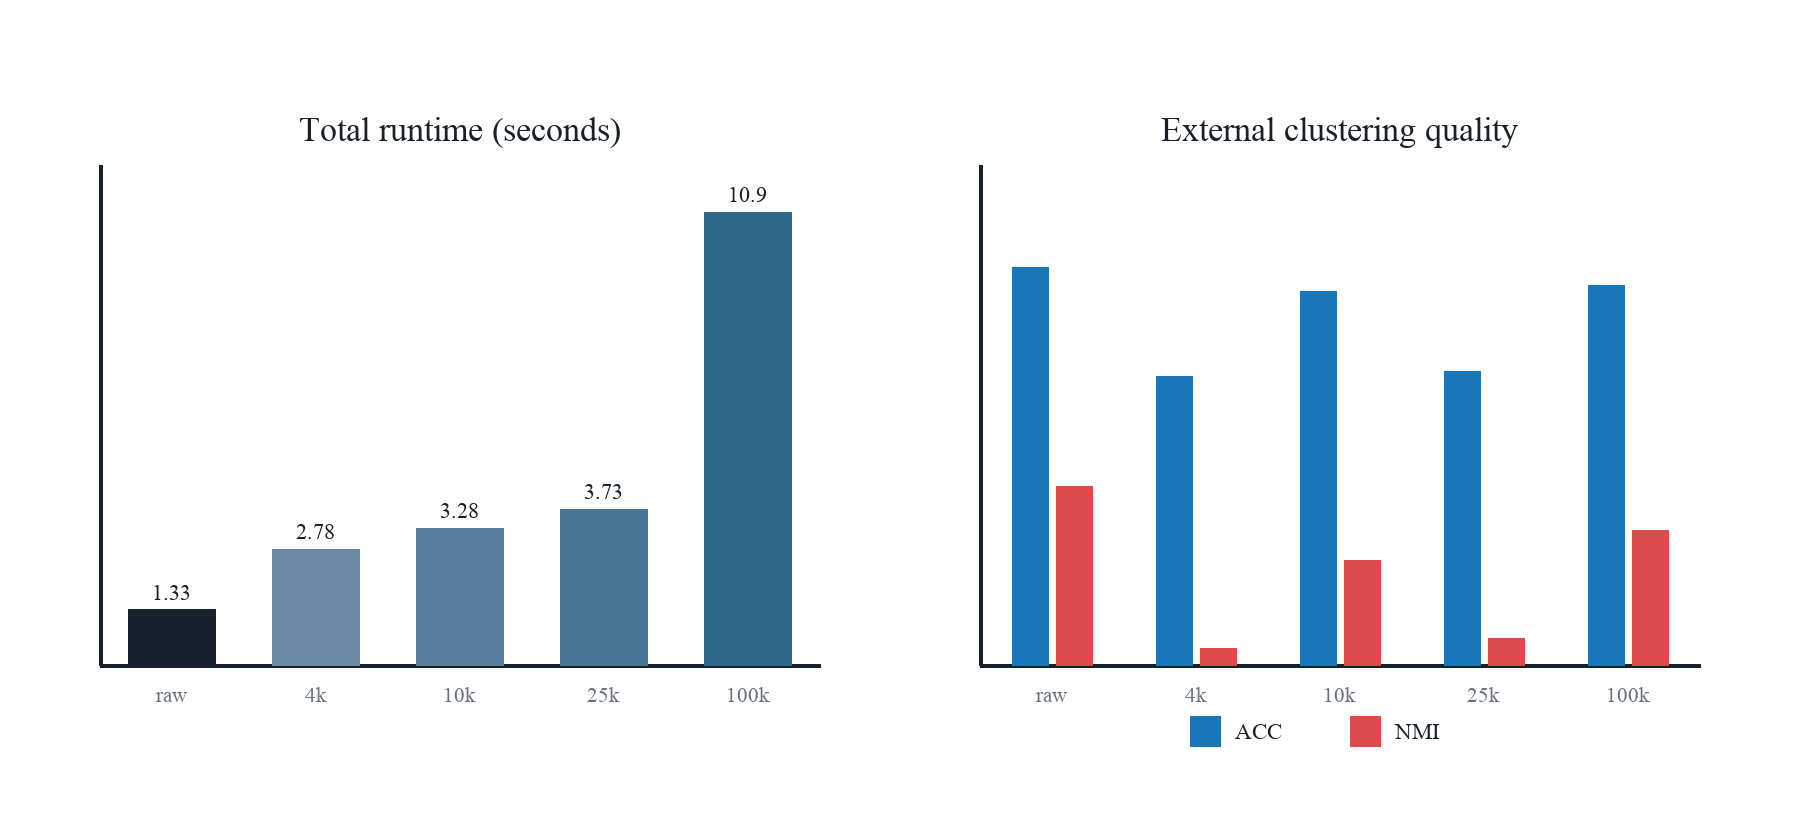
\includegraphics[width=\textwidth]{Figures/kpp_results.png}
    \caption{زمان کل و کیفیت برای افرازهای اولیه‌ی مختلف روی
        \lr{Gisette}.}
    \label{fig:kpp-results}
\end{figure}

افراز اولیه تعداد ادغام‌های هسته را کاهش می‌دهد، اما هزینه‌ی اجرای
\lr{KMeans} مقدماتی باعث شد زمان کل در همه‌ی حالت‌ها از روش اصلی بیشتر
شود. هزینه‌ی تقریبی داخلی کمی کاهش یافت، ولی \lr{ACC} و \lr{NMI} بدتر

\section{نتیجه‌گیری کلی}

دستاورد این مرحله بیش از آن‌که یک الگوریتم بهتر باشد، تبدیل دو ایده‌ی اولیه
به فرضیه‌های قابل‌آزمون و مشخص کردن حالت‌های شکست آن‌هاست. روش elbow قابل اتکا نیست. افراز اولیه‌ی فعلی نیز در آزمایش
انجام‌شده زمان کل و کیفیت بیرونی را بهبود نداد. در مقابل، مطالعه‌ی منابع
تاریخی و جدید، ایجاد ابزارهای تکرارپذیر، بهبود زمان و ساخت صفحات
تعاملی، پایه‌ی روشنی برای مرحله‌ی بعد پروژه فراهم کرده است.
